\documentclass[12pt,aspectratio=169]{beamer}

\usetheme[
    sectionpage=progressbar,
    subsectionpage=progressbar,
    progressbar=frametitle
]{metropolis}

\usepackage[utf8]{inputenc}
\usepackage[spanish]{babel}
\usepackage{graphicx}

\title{Introducción a la Optimización para Invertir en la Bolsa}
\author{Luis Biedma}
\date{29/09/2018}

\begin{document}

\maketitle

\section{Introducción}

\begin{frame}{Introducción}
Imaginemos que tenemos que armar un desayuno nutritivo con los siguientes elementos:

\begin{center}
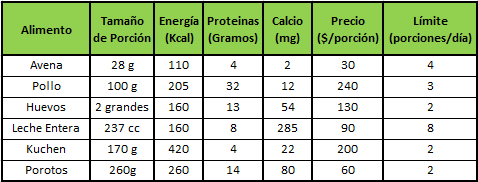
\includegraphics[width=.8\paperwidth]{desayuno.png}
\end{center}
\end{frame}

\begin{frame}{Introducción}
Un problema similar a éste tenía Leonid Kantorovich en los '40.

\begin{center}
\uncover<2>{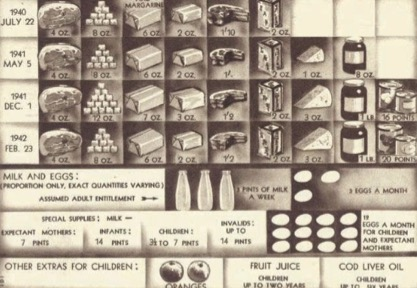
\includegraphics[width=.5\paperwidth]{rations.jpg}}
\end{center}
\end{frame}

\begin{frame}{Qué es la optimización?}
\begin{itemize}
\item Maximizar o minimizar una función (objetivo, costo, pérdida)...
\item ... relativo a algún conjunto (restricciones)

\end{itemize}


\begin{center}
	\uncover<2>{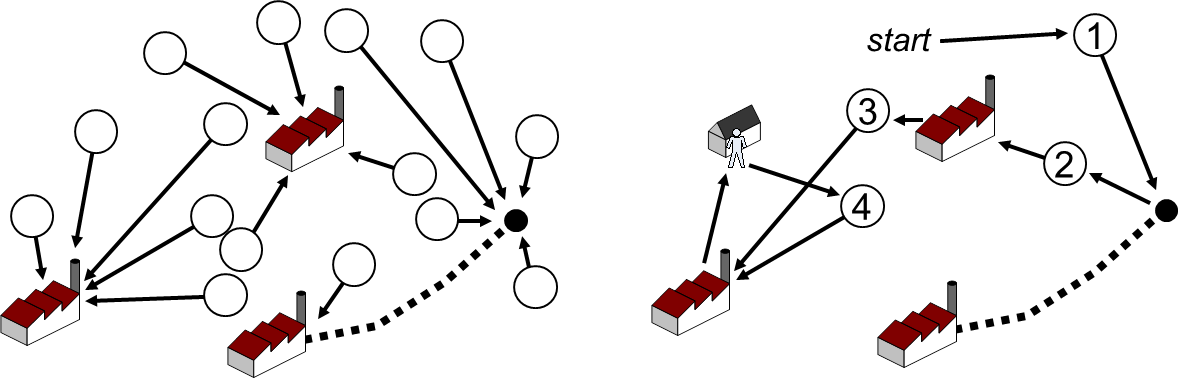
\includegraphics[width=.5\paperwidth]{optimization.png}}
\end{center}

\end{frame}

\section{Teoría Moderna de Portafolios}

\section{Notebook}

\section{Conclusiones}
\begin{frame}
\textbf{Control de daños:}

\begin{itemize}
\item Le ganamos al mercado!
\item Es posible armar una estrategia de esta manera? Variables enteras...
\item Comisiones...
\end{itemize}

\textbf{Espacio para mejorar:}

\begin{itemize}
\item Ganancia esperada.
\item Reinforcement learning.
\item Sentiment analysis
\item Etece, etece, etece...
\end{itemize}
\end{frame}

\begin{frame}
\centering
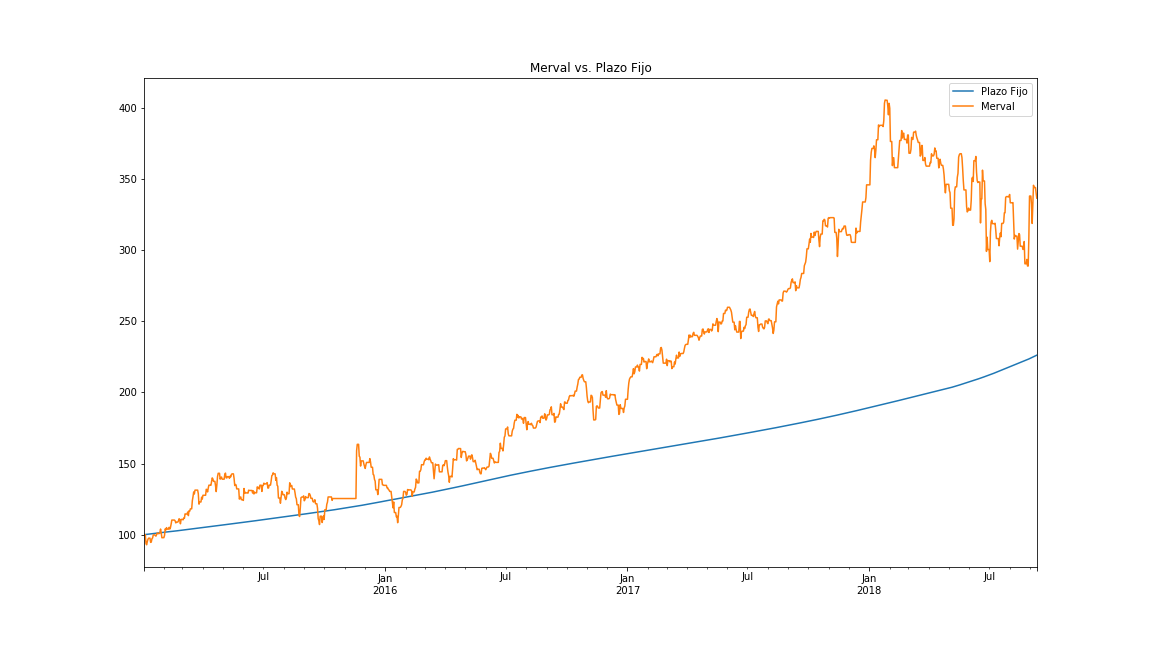
\includegraphics[height=.9\paperheight]{plazofijovsmerval.png}
\end{frame}

\end{document}